\documentclass[conference]{IEEEtran}

\usepackage[T1]{fontenc}
\usepackage{microtype}
\usepackage{graphicx}
\usepackage{booktabs}
\usepackage{tabularx}
\usepackage{array}
\usepackage{amsmath,amssymb}
\usepackage{xcolor}
% Visual system: low-saturation accents with light fills for figures and callouts.
\definecolor{SignalInk}{HTML}{40566F}
\definecolor{SignalLine}{HTML}{8493A1}
\definecolor{SignalBlue}{HTML}{E8EFF4}
\definecolor{SignalSage}{HTML}{E7EFEB}
\definecolor{SignalSand}{HTML}{F3EDE2}
\usepackage{hyperref}
\usepackage{enumitem}
\usepackage{tikz}
\usetikzlibrary{arrows.meta,positioning,shapes.geometric}

\hypersetup{
  colorlinks=true,
  linkcolor=SignalInk,
  citecolor=SignalInk,
  urlcolor=SignalInk,
  pdftitle={Indoor Positioning from Wi-Fi Signal Strength Fingerprints},
  pdfauthor={}
}
\setlength{\parskip}{0pt}
\setlist[itemize]{leftmargin=1.5em,itemsep=0.2em,topsep=0.3em}
\renewcommand{\arraystretch}{1.15}

\title{Indoor Positioning from Wi-Fi Signal Strength Fingerprints}
\author{}
\date{}

\begin{document}
\maketitle
\begin{abstract}
Reliable indoor localization is difficult when satellite positioning is unavailable, while Wi-Fi access points provide sparse signal observations whose patterns vary with location. This paper presents and evaluates a fingerprint-based localization pipeline using the UJIIndoorLoc multi-building, multi-floor dataset. Each measurement contains received signal strength indicator (RSSI) readings from 520 wireless access points (WAPs), together with building, floor, and two-dimensional coordinate labels. A sentinel-aware preprocessing method separates missing observations from signal strength, fits per-access-point scaling statistics on training data only, and augments the readings with binary detection masks and six row-level signal summaries. The resulting representation contains 1,046 predictors. Three independent Random Forest estimators predict building identity, floor code, and coordinates. Model configurations are selected on a grouped internal development split; the supplied 1,111-record validation partition is kept for final evaluation. On this partition, building accuracy is 99.73\%, floor accuracy is 88.93\%, and mean Euclidean coordinate error is 11.58 recorded coordinate units. Building and floor are jointly correct for 88.75\% of records. The results show that the three localization targets differ in difficulty and that coordinate error tends to rise when the predicted floor is incorrect. Because records and coordinate values may recur across partitions, and authoritative coordinate reference metadata is absent, these measurements characterize the supplied evaluation partition and must be interpreted under the coordinate assumptions documented by the dataset pipeline rather than as evidence of performance at an independent site.
\end{abstract}
\begin{IEEEkeywords}
indoor positioning, Wi-Fi fingerprinting, RSSI, Random Forest, classification, coordinate regression, UJIIndoorLoc
\end{IEEEkeywords}

\section{Introduction}
Indoor satellite positioning is often unavailable or unreliable, while Wi-Fi access points provide signal observations that vary across locations. A Wi-Fi fingerprint is a vector of received signal strengths measured from a set of access points. The project treats each row as a fingerprint and predicts three related location targets: building identity, floor identity, and two-dimensional position.

\subsection{Related work}
Wi-Fi fingerprinting compares a live RSSI vector with a radio map collected at known locations. Deterministic methods such as nearest-neighbor matching select the closest stored fingerprints, whereas probabilistic methods model the likelihood of signal observations at candidate locations. A controlled comparison by Dawes and Chin found that nearest-neighbor variants can perform well with reduced signal dimensions, while also showing that transient access points and signal variability affect accuracy; they emphasize that performance depends on the test environment \cite{dawes2011}. He and Chan review extensions that use spatial and temporal patterns or combine Wi-Fi with motion and other sensors to improve localization, at the cost of added data or sensing requirements \cite{hechan2016}.

On UJIIndoorLoc, Song \emph{et al.} proposed CNNLoc, which combines a stacked autoencoder with a one-dimensional CNN for building and floor classification and coordinate estimation \cite{song2019}. This learned representation is a more complex alternative to direct fingerprint matching and conventional tabular models. The present study evaluates Random Forest models on an explicit engineered feature table and keeps building, floor, and coordinate predictions separate. Since this project does not test nearest-neighbor, probabilistic, or CNN baselines under the same split, the results establish performance for the selected pipeline only; they do not rank it against those published methods. Differences in partitions and metrics also prevent direct comparison of reported scores.

The implemented system uses a shared, deterministic feature preparation pipeline followed by three independent tabular estimators. This structure follows the project specification: absent access points are represented consistently, signal-density summaries are added, classification predicts building and floor, and regression predicts coordinates. The UJIIndoorLoc database was introduced for multi-building and multi-floor WLAN fingerprint-based localization research \cite{torres2014,uci}.

The central modeling question is: how well can a Wi-Fi fingerprint predict each location target under the supplied data partition when the transformations and model settings are learned without using the final held-out labels? The three prediction targets are evaluated separately because building class, floor code, and coordinates have different label types and error measures. Their predictions are then joined to describe whether their errors coincide on the same records.

\section{Data and problem definition}
\subsection{Dataset and observed schema}
The repository contains the UJIIndoorLoc training/reference file and supplied validation file. The observed training file has 19,937 rows and 529 columns; the supplied validation file has 1,111 rows and 529 columns. Each file contains 520 WAP signal columns, four targets (building ID, floor, longitude, latitude), and five metadata fields (space ID, relative position, user ID, phone ID, timestamp). Dataset documentation describes measurements from multiple buildings and floors at Universitat Jaume I \cite{uci,torres2014}.

Table~\ref{tab:schema} summarizes how these columns are used. A row is a measurement record, not a sequence model input. The WAP feature names are ordered by their numeric suffix; row identifiers and collection metadata are carried through for traceability and split checks, not supplied to the estimators.

\begin{table}[!t]
\centering
\caption{Observed data groups and their roles in the pipeline.}
\label{tab:schema}
\begin{tabularx}{\columnwidth}{p{0.23\columnwidth} p{0.16\columnwidth} X}
\toprule
Column group & Count & Pipeline role \\
\midrule
WAP RSSI fields & 520 & Inputs; sentinel-aware scaling, presence masks, plus row summaries. \\
Building and floor & 2 & Classification targets; never included in the predictor allowlist. \\
Longitude and latitude & 2 & Joint regression targets; never included in the predictor allowlist. \\
Collection/location metadata & 5 & Retained for auditing, grouping, and interpretation; excluded from predictors. \\
\bottomrule
\end{tabularx}
\end{table}

The targets are treated as three separate prediction tasks. Building and floor are integer-coded classes. Longitude and latitude are modeled jointly as two numeric outputs. Floor codes are reused across buildings, so floor classification predicts the floor code alone; it is not a single combined building--floor class. The held-out validation file contains zero placeholders for \path{SPACEID}, \path{RELATIVEPOSITION}, and \path{USERID}; these metadata fields are not used as model inputs.

\subsection{Signal encoding and quality checks}
The notebooks discover WAP columns by matching the \texttt{WAP} prefix and numeric suffix. In both source files, the value \texttt{100} is the dominant missing-signal sentinel; other observed signal values are non-positive and are interpreted as dBm. Training data has an average absent-signal fraction of about 96.54\% across WAP entries, compared with about 96.83\% in the supplied held-out data. There are no blank cells in the checked files. The training file contains 637 exact duplicate rows and 76 rows with no detected access points; these rows were counted and retained. The held-out file has no exact duplicate rows or all-absent-signal rows in the recorded checks. A full-row hash comparison found no exact raw-row overlap between the two supplied files.

The class counts are not uniform. There are three building classes and five floor codes in the training data, while floor 4 has substantially fewer examples than floors 0--3. The validation partition also has only 39 floor-4 examples. This imbalance is relevant when interpreting raw accuracy: a model can achieve high overall accuracy while still making a disproportionate number of errors on a small class.

\section{Data partitioning and leakage controls}
\subsection{Development split}
The 19,937-row training/reference file is divided with \texttt{GroupShuffleSplit} using a 20\% internal validation fraction and random seed 42. Groups are defined by the composite building, floor, and space identifiers. This gives 16,085 internal-training rows and 3,852 internal-validation rows; the two subsets have disjoint composite group sets. The original supplied validation file remains a separate 1,111-row held-out partition.

The split is made on a composite key, not on individual rows. The notebook verifies 588 unique groups in internal training and 147 in internal validation, with no group shared between them. This prevents the same building/floor/space key from being split across these two development subsets. It also verifies unique row IDs across the internal split artifacts.

\subsection{Why an internal validation set is used}
The supplied \texttt{validationData.csv} is reserved as the final evaluation partition. A second, internal validation subset is created from \texttt{trainingData.csv} because model selection still requires a labelled set on which candidate settings can be compared. If tuning choices were made by repeatedly checking the supplied held-out scores, information from the final evaluation labels would influence the chosen model and the reported held-out score would become optimistically biased. The internal validation set handles model selection; the supplied validation set estimates the performance of the frozen configuration under the project's chosen split.

The internal validation rows are not used to fit the scaler or estimator. They are used to score candidate configurations and choose among them. The selected estimator is then fit on the internal-training rows and applied once to the supplied held-out rows. This evaluation estimates performance for the supplied partition; it is not an independent external-site test, and it does not guarantee that signal fingerprints or 2D coordinates are unique across all partitions.

\subsection{Predictor allowlist and fitting boundaries}
The shared predictor matrix contains 1,046 columns: 520 scaled RSSI values, 520 binary detection indicators, and six signal summaries. Target labels and all identifiers/collection metadata are retained for verification and analysis but excluded from prediction. Each task notebook independently reconstructs and validates the feature allowlist from the feature table schema. RSSI scaling parameters are learned only from observed values in internal training and reused unchanged on internal validation and held-out data. The held-out file is loaded only after the task-specific configuration is frozen.

These checks prevent direct target or identifier leakage and prevent transformation statistics or hyperparameter selection from using held-out targets. They do not establish a stricter unseen-fingerprint or unseen-position evaluation. Comparing the exported WAP signal vectors shows eight distinct exact fingerprints shared between internal training and internal validation, and none shared between internal training and the supplied held-out partition. Exact coordinate pairs recur across both comparisons: 62 between internal training and internal validation, and eight between internal training and supplied held-out data. Thus, a complete row or fingerprint can be absent from a split while the same coordinate is represented in training. A grouped split by building/floor/space also does not assert independence of every underlying signal pattern.

\section{Preprocessing and feature engineering}
\subsection{Missing-aware RSSI transformation}
For each WAP, the sentinel value 100 is converted to an absent observation, not treated as a signal strength. For WAP \(j\), the internal-training observed values define the mean \(\mu_j\) and population standard deviation \(\sigma_j\). Observed values are standardized as
\[
 z_{ij}=\frac{r_{ij}-\mu_j}{\sigma_j},
\]
where \(r_{ij}\) is the RSSI of sample \(i\) for WAP \(j\). A zero or undefined scale is replaced with one. Absent values receive a finite per-WAP fill below the minimum standardized training observation; a separate binary indicator remains authoritative for whether that WAP was actually seen. For WAPs with no observed internal-training samples, the transformation uses the observed internal-training RSSI pool as a fallback. No statistic is estimated from internal validation or held-out data.

\subsection{Signal summary features}
Six row-level features supplement the 1,040 WAP-specific inputs:
\begin{itemize}
  \item \texttt{n\_heard}: number of detected access points;
  \item \texttt{max\_rssi\_dbm}: strongest observed signal;
  \item \texttt{mean\_rssi\_dbm} and \texttt{std\_rssi\_dbm}: mean and standard deviation among detected signals;
  \item \texttt{n\_strong}: number of observed signals stronger than \(-70\) dBm; and
  \item \texttt{top1\_ap\_index}: zero-based index of the strongest WAP.
\end{itemize}
Rows with no detected WAP use explicit finite summary values and a strongest-access-point index of \(-1\). The canonical output tables also retain row ID, source partition, original metadata, and all targets for traceability and evaluation joins. These retained fields are not part of the predictor allowlist.

The resulting feature row has 1,046 values. The WAP signal columns preserve relative per-access-point signal variation after normalization; the binary masks separately represent observation availability; the six summaries provide compact indicators of how many signals were detected and their overall strength. The explicit feature allowlist makes this predictor boundary inspectable and prevents a row key, source label, target, or metadata field from entering a model by accident.

\begin{figure}[!t]
\centering
\resizebox{\columnwidth}{!}{%
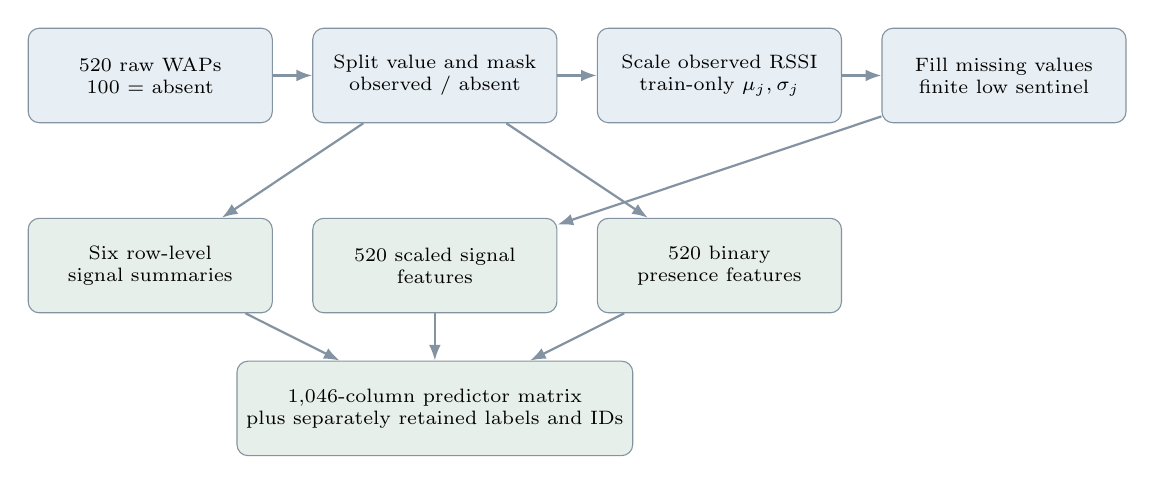
\begin{tikzpicture}[
  node distance=6mm and 5mm,
  pbox/.style={draw=SignalLine,rounded corners,align=center,minimum width=31mm,minimum height=12mm,fill=SignalBlue,font=\scriptsize},
  gbox/.style={draw=SignalLine,rounded corners,align=center,minimum width=31mm,minimum height=12mm,fill=SignalSage,font=\scriptsize},
  arrow/.style={-{Latex[length=2mm]},thick,draw=SignalLine}
]
\node[pbox] (raw) {520 raw WAPs\\100 = absent};
\node[pbox,right=of raw] (mask) {Split value and mask\\observed / absent};
\node[pbox,right=of mask] (scale) {Scale observed RSSI\\train-only $\mu_j,\sigma_j$};
\node[pbox,right=of scale] (fill) {Fill missing values\\finite low sentinel};
\node[gbox,below=12mm of mask] (signals) {520 scaled signal\\features};
\node[gbox,right=of signals] (masks) {520 binary\\presence features};
\node[gbox,left=of signals] (summary) {Six row-level\\signal summaries};
\node[gbox,below=of signals] (matrix) {1,046-column predictor matrix\\plus separately retained labels and IDs};
\draw[arrow] (raw) -- (mask);
\draw[arrow] (mask) -- (scale);
\draw[arrow] (scale) -- (fill);
\draw[arrow] (fill) -- (signals);
\draw[arrow] (mask) -- (masks);
\draw[arrow] (mask) -- (summary);
\draw[arrow] (signals) -- (matrix);
\draw[arrow] (masks) -- (matrix);
\draw[arrow] (summary) -- (matrix);
\end{tikzpicture}%
}
\caption{Feature construction from sparse WAP measurements. The mask preserves missingness explicitly, while all learned scaling values come from internal training only.}
\label{fig:feature-construction}
\end{figure}

\section{Modeling methods}
\subsection{Random Forest rationale}
The project uses Random Forests for the three localization tasks. A Random Forest aggregates decision trees fit on bootstrap samples and randomized feature subsets \cite{breiman2001}. At each split, a tree considers a subset of candidate predictors rather than always comparing all 1,046 inputs. This decorrelates the trees; bootstrapping creates variation in their training examples. For classification the forest returns the most-voted class, while for regression it averages tree predictions for each output coordinate:
\[
\hat{c}(\mathbf{x})=\operatorname{mode}_{b=1,\ldots,B} h_b(\mathbf{x}),\qquad
\hat{\mathbf{y}}(\mathbf{x})=\frac{1}{B}\sum_{b=1}^{B}\mathbf{g}_b(\mathbf{x}).
\]
Here, \(B\) is the number of trees, \(h_b\) is a class prediction, and \(\mathbf{g}_b\) is a two-coordinate prediction. Tree count, depth, leaf size, and feature subsampling shape the bias/variance trade-off: more trees stabilize the aggregation, while depth and leaf size control how finely individual trees partition the feature space. Class weights alter the contribution of floor classes during tree fitting. The project benchmarks Random Forest configurations only; it does not claim superiority over untested alternatives.

All task implementations fix the random seed for reproducibility and run trees with parallel jobs. The selected parameter settings below are specific to this dataset and split. They are not universal defaults or evidence that these models are optimal beyond the tested grids.

\subsection{Building classification}
The building estimator is a \texttt{RandomForestClassifier} with \texttt{BUILDINGID} as its target. The notebook fits a 100-tree baseline first, then evaluates an 18-configuration grid on the internal validation rows. The grid varies tree count over \(\{100,200,300\}\), maximum depth over \(\{\text{unlimited},20,30\}\), and minimum leaf size over \(\{1,2\}\). Each candidate is fit only on internal training. Internal-validation accuracy is the primary selection score, with macro F1 breaking ties. The selected setting is 100 trees, unlimited depth, and minimum leaf size one; it matches the recorded baseline setting. After selection is frozen, the estimator is fit on internal training and scored on the held-out file. Evaluation includes accuracy, macro F1, and a confusion matrix over the building labels observed in internal training.

\subsection{Floor classification}
The floor estimator is a separate \texttt{RandomForestClassifier} with \texttt{FLOOR} as its target. The observed floor-label mapping is formed from internal-training labels in ascending numeric order and reused for internal validation and held-out evaluation. Building ID and all metadata are excluded from predictors; therefore, this task predicts the floor code alone, not a building--floor pair. The model uses balanced class weights to reduce the influence of the uneven class frequencies during tree construction.

The eight-candidate grid crosses tree counts \(\{150,300\}\), depths \(\{\text{unlimited},30\}\), and leaf sizes \(\{1,2\}\), with \texttt{max\_features=sqrt} fixed. A 100-tree baseline is also reported. Internal-validation accuracy selects the configuration; macro F1 is a class-balanced diagnostic and is included in deterministic tie-breaking. The chosen setting has 150 trees, unlimited depth, minimum leaf size one, \texttt{max\_features=sqrt}, and balanced class weights. The held-out confusion matrix uses the fixed internal-training class list, so classes do not disappear when a partition has few examples.

\subsection{Coordinate regression}
The coordinate estimator is a multi-output \texttt{RandomForestRegressor} that predicts longitude and latitude together. Its explicit predictor allowlist excludes both coordinate targets and all metadata identifiers. The baseline uses 100 trees, unlimited depth, and leaf size one. Ten candidates then vary tree count (100, 150, or 200), maximum depth (unlimited or 50 for selected candidates), minimum leaf size (one or two), and feature subsampling (all features, \texttt{sqrt}, or 0.5). Each candidate is fit on internal training and scored on internal validation by mean Euclidean distance. The selected configuration uses 150 trees, unlimited depth, minimum leaf size one, and \texttt{max\_features=0.5}. It reduces the internal-validation mean Euclidean error from 9.26 for the baseline to 8.58 coordinate units.

Table~\ref{tab:coordinate-search} reports every tested coordinate configuration, ranked by the internal-validation selection metric. The first row is the selected configuration. This table makes clear that selection was performed over the recorded ten candidates rather than over an unreported search.

\begin{table}[!t]
\centering
\caption{Coordinate regressor search results on internal validation, ranked by mean Euclidean error.}
\label{tab:coordinate-search}
\small
\resizebox{\columnwidth}{!}{%
\begin{tabular}{rrrrr}
\toprule
Trees & Maximum depth & Minimum leaf & Features per split & Mean Euclidean error \\
\midrule
150 & unlimited & 1 & 0.5 & 8.5786 \\
200 & unlimited & 1 & sqrt & 8.6567 \\
150 & unlimited & 1 & sqrt & 8.6749 \\
150 & 50 & 1 & all & 9.1912 \\
150 & unlimited & 1 & all & 9.2004 \\
200 & unlimited & 1 & all & 9.2024 \\
200 & 50 & 1 & all & 9.2030 \\
100 & unlimited & 1 & all & 9.2561 \\
150 & unlimited & 2 & all & 9.4175 \\
200 & unlimited & 2 & all & 9.4294 \\
\bottomrule
\end{tabular}%
}
\end{table}

The coordinate notebook labels coordinates as EPSG:3857 projected metres. The repository does not provide authoritative CRS metadata, so all coordinate-unit results below must be read as values under the notebook's stated EPSG:3857 assumption. They are not corrected for projection scale and should not be interpreted as verified ground-distance errors.

\begin{table}[!t]
\centering
\caption{Task-specific search spaces and selection criteria. All candidates use the shared internal-training and internal-validation partitions.}
\label{tab:tuning-design}
\begin{tabularx}{\columnwidth}{p{0.16\columnwidth} p{0.40\columnwidth} p{0.12\columnwidth} X}
\toprule
Task & Parameters varied & Candidates & Selection rule \\
\midrule
Building & Trees: 100, 200, 300; depth: unlimited, 20, 30; leaf: 1, 2 & 18 & Accuracy; macro F1 tie-break \\
Floor & Trees: 150, 300; depth: unlimited, 30; leaf: 1, 2; features fixed to sqrt; balanced class weights & 8 & Accuracy; macro F1 and deterministic parameter-order tie-break \\
Coordinates & Trees: 100, 150, 200; depth: unlimited or 50; leaf: 1 or 2; features: all, sqrt, or 0.5 in the tested combinations & 10 & Lowest mean Euclidean error \\
\bottomrule
\end{tabularx}
\end{table}

\section{Evaluation measures}
For classification, accuracy is the proportion of correct predictions,
\[
 \mathrm{Accuracy}=\frac{1}{n}\sum_{i=1}^{n}\mathbb{1}(y_i=\hat y_i),
\]
while macro F1 is the arithmetic mean of per-class F1 scores,
\[
 \mathrm{Macro\ F1}=\frac{1}{K}\sum_{k=1}^{K}
 \frac{2\,\mathrm{Precision}_k\,\mathrm{Recall}_k}
 {\mathrm{Precision}_k+\mathrm{Recall}_k}.
\]
Each of the \(K\) classes contributes equally to macro F1, so a sparse class is not overwhelmed by larger classes. The confusion matrix reports true labels by predicted labels. The floor confusion matrix is useful for examining neighboring-code confusions and the smaller number of floor-4 examples.

For coordinate predictions \((\hat{x}_i,\hat{y}_i)\) against observed coordinates \((x_i,y_i)\), axis-specific mean absolute error is
\[
 \mathrm{MAE}_{x}=\frac{1}{n}\sum_{i=1}^{n}|x_i-\hat{x}_i|,\qquad
 \mathrm{MAE}_{y}=\frac{1}{n}\sum_{i=1}^{n}|y_i-\hat{y}_i|.
\]
The two-dimensional error is \(d_i=\sqrt{(x_i-\hat{x}_i)^2+(y_i-\hat{y}_i)^2}\); the report gives its mean and median. These are computed in the coordinate units recorded by the regression pipeline.

\section{Results}
\subsection{Task-level performance}
Table~\ref{tab:results} reports internal-validation results used during development and final supplied held-out results. The held-out column is the main performance estimate; the internal-validation column reflects the model-selection data and is expected to be more favorable because candidates were ranked there. The supplied held-out evaluation is performed only after the selected configuration is frozen.

\begin{table}[!t]
\centering
\caption{Task metrics by split. Coordinate metrics use the notebook's stated EPSG:3857 metre assumption.}
\label{tab:results}
\small
\begin{tabularx}{\columnwidth}{>{\raggedright\arraybackslash}p{0.22\columnwidth} >{\centering\arraybackslash}p{0.15\columnwidth} >{\centering\arraybackslash}p{0.15\columnwidth} X}
\toprule
Task & Internal validation & Held-out validation & Selected model configuration \\
\midrule
Building accuracy & 99.95\% & 99.73\% & RF: 100 trees, unlimited depth, leaf size 1 \\
Building macro F1 & 99.95\% & 99.71\% & same configuration \\
Floor accuracy & 96.42\% & 88.93\% & RF: 150 trees, unlimited depth, leaf size 1, \texttt{sqrt}, balanced weights \\
Floor macro F1 & 96.78\% & 87.27\% & same configuration \\
Longitude MAE & 5.91 & 8.10 & RF regressor: 150 trees, unlimited depth, leaf size 1, max features 0.5 \\
Latitude MAE & 5.06 & 6.81 & same configuration \\
Mean Euclidean error & 8.58 & 11.58 & same configuration \\
Median Euclidean error & 6.31 & 7.49 & same configuration \\
\bottomrule
\end{tabularx}
\end{table}

For building, tuning retains the baseline setting. Floor accuracy rises from 96.21\% to 96.42\% on internal validation, while coordinate mean Euclidean error falls from 9.26 to 8.58 units. Held-out floor and coordinate results are lower than these selected internal-validation scores; the held-out data was not used to choose configurations.

\begin{figure}[!t]
  \centering
  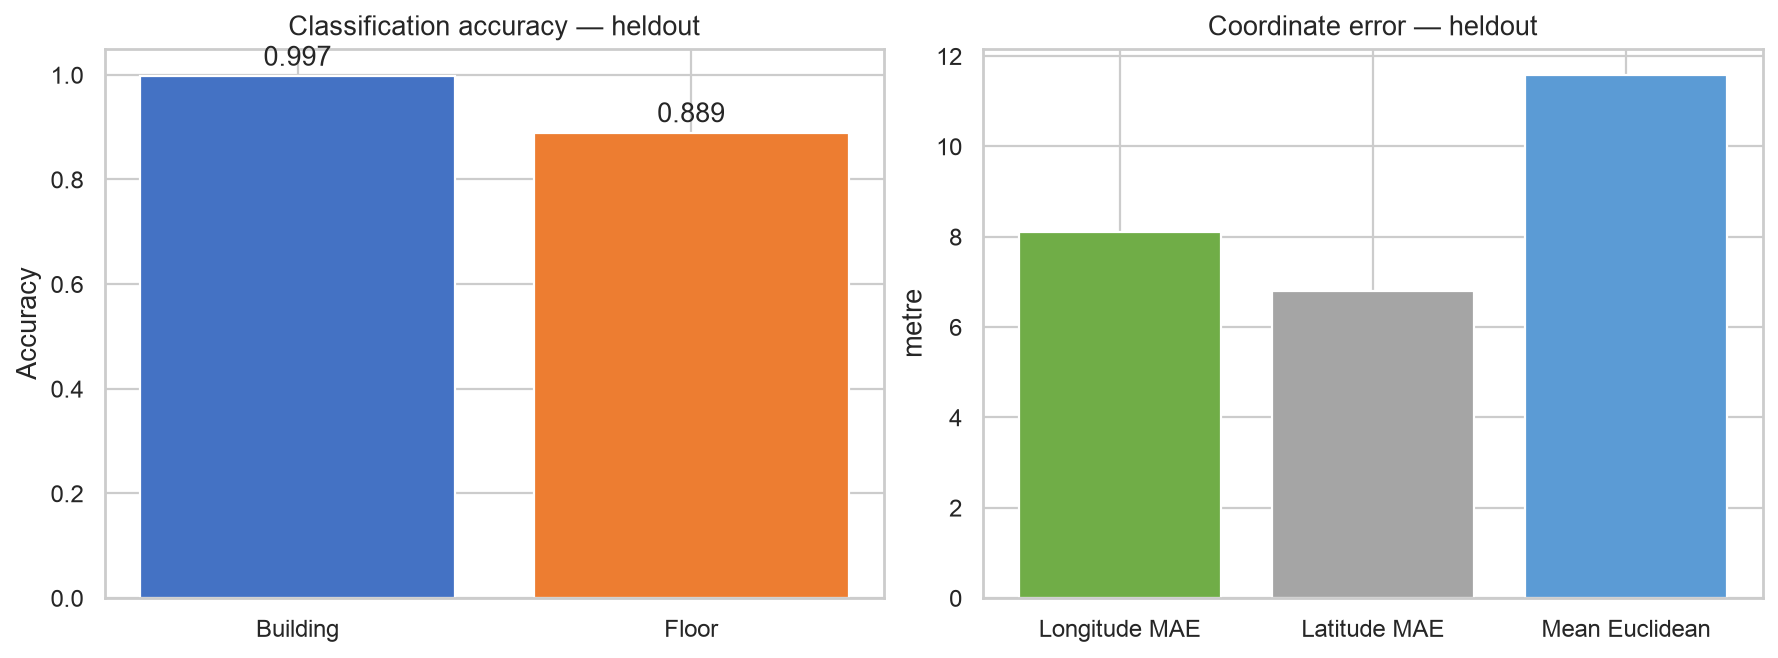
\includegraphics[width=\columnwidth]{../data/figures/ml_05_heldout_metric_comparison.png}
  \caption{Held-out classification accuracy and coordinate error on their task-specific scales. The left and right panels have different metrics and units; bar heights should not be compared across panels.}
  \label{fig:metric-comparison}
\end{figure}

\subsection{Building and floor classification}
Building classification correctly predicts 1,108 of 1,111 held-out rows. The building confusion matrix contains only three errors: one building-0 record and one building-1 record are predicted as a neighboring code, and one building-1 record is predicted as building 2. The floor classifier correctly predicts 988 of 1,111 rows. Most floor errors are between neighboring codes, and floor 4 has the smallest support. Table~\ref{tab:floor-recall} reports per-code support, correct predictions, and recall derived from the held-out confusion matrix.

\begin{table}[!t]
\centering
\caption{Held-out floor recall by true floor code.}
\label{tab:floor-recall}
\begin{tabular}{rrrr}
\toprule
True floor & Support & Correct & Recall \\
\midrule
0 & 132 & 119 & 90.15\% \\
1 & 462 & 401 & 86.80\% \\
2 & 306 & 279 & 91.18\% \\
3 & 172 & 162 & 94.19\% \\
4 & 39 & 27 & 69.23\% \\
\bottomrule
\end{tabular}
\end{table}

The largest single off-diagonal floor count is true floor 1 predicted as floor 2 (49 records), followed by true floor 4 predicted as floor 3 (10 records). Since floor codes are modeled as nominal classes, the classifier does not explicitly penalize a two-floor error more than a one-floor error; the matrix is needed to understand the structure behind accuracy and macro F1. Figure~\ref{fig:confusions} presents the held-out building and floor matrices, and Figure~\ref{fig:floor-cm} shows the floor counts at higher size.

\begin{figure}[!t]
  \centering
  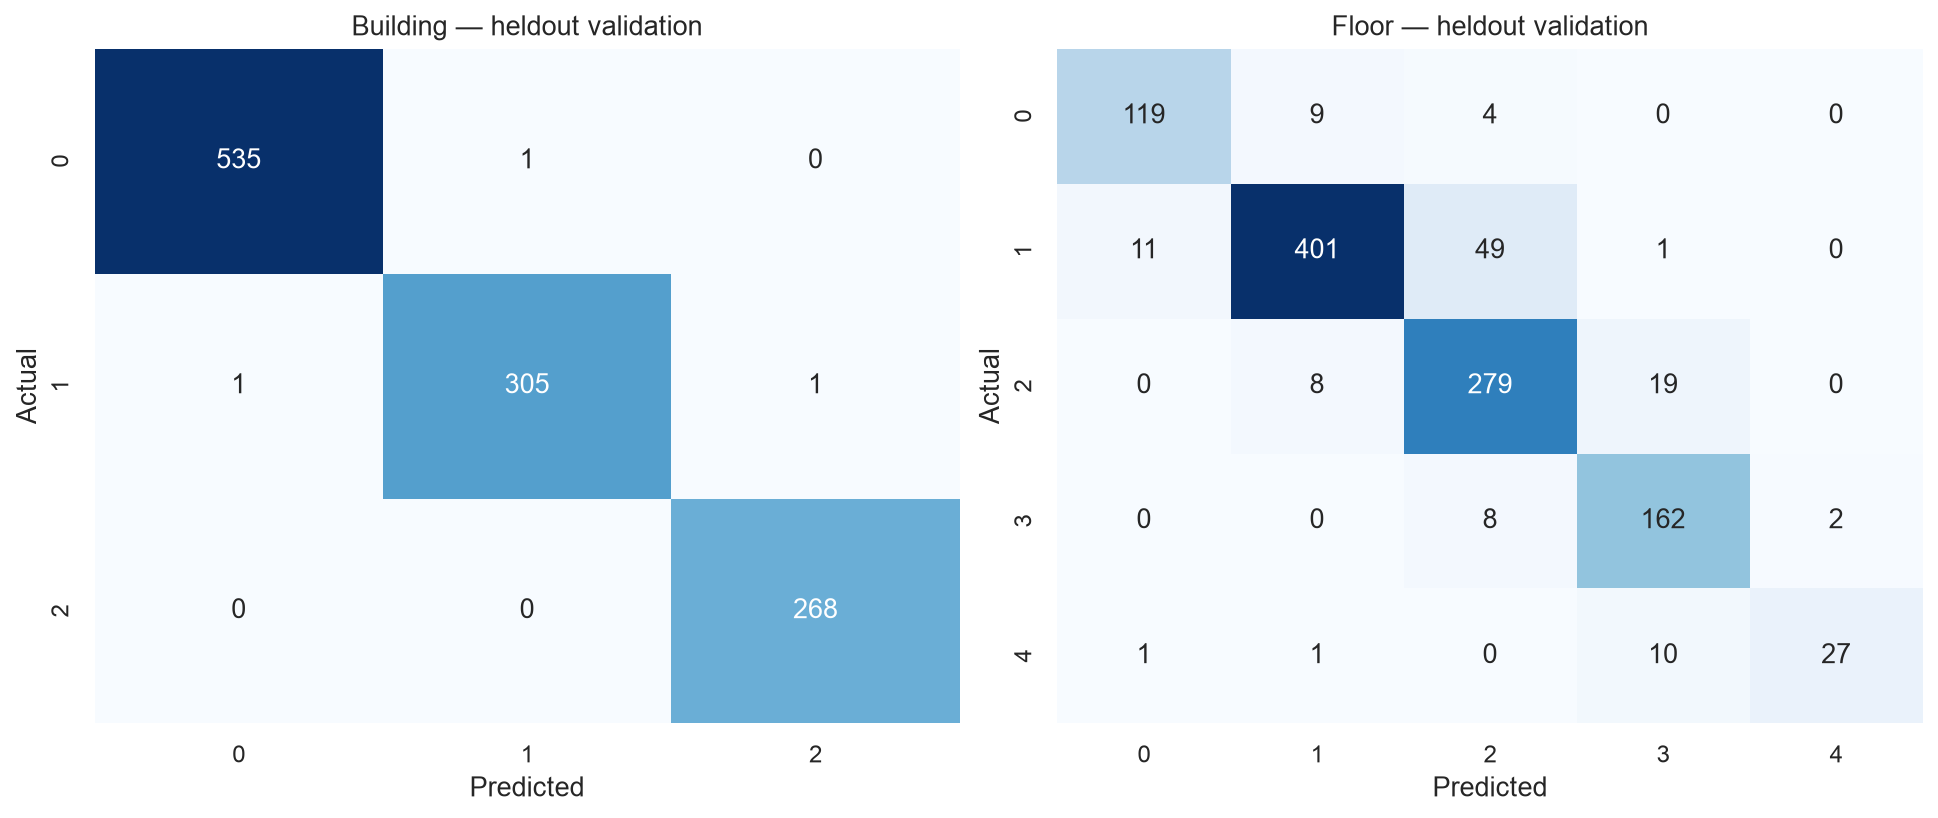
\includegraphics[width=0.91\columnwidth]{../data/figures/ml_05_heldout_confusion_matrices.png}
  \caption{Held-out building and floor confusion matrices regenerated from the integrated row-aligned predictions.}
  \label{fig:confusions}
\end{figure}

\subsection{Coordinate regression}
The held-out longitude-axis MAE is 8.10 coordinate units, latitude-axis MAE is 6.81, mean Euclidean error is 11.58, and median Euclidean error is 7.49. The internal validation mean Euclidean error is 8.58. The increase on the supplied held-out partition indicates that internal-validation performance should not be substituted for the final estimate. Figure~\ref{fig:errormap} shows held-out samples in coordinate space colored by prediction error, using the recorded coordinate values without a basemap or reprojection.

The held-out error distribution is right-skewed: the median is below the mean, and a smaller set of larger errors raises the mean. The 75th and 95th percentiles are 13.68 and 36.21 coordinate units, respectively. This distinction matters because the mean alone hides the error tail. Axis MAEs summarize residuals separately by coordinate component, while Euclidean error measures the combined two-dimensional displacement for each record.


\begin{figure}[!t]
  \centering
  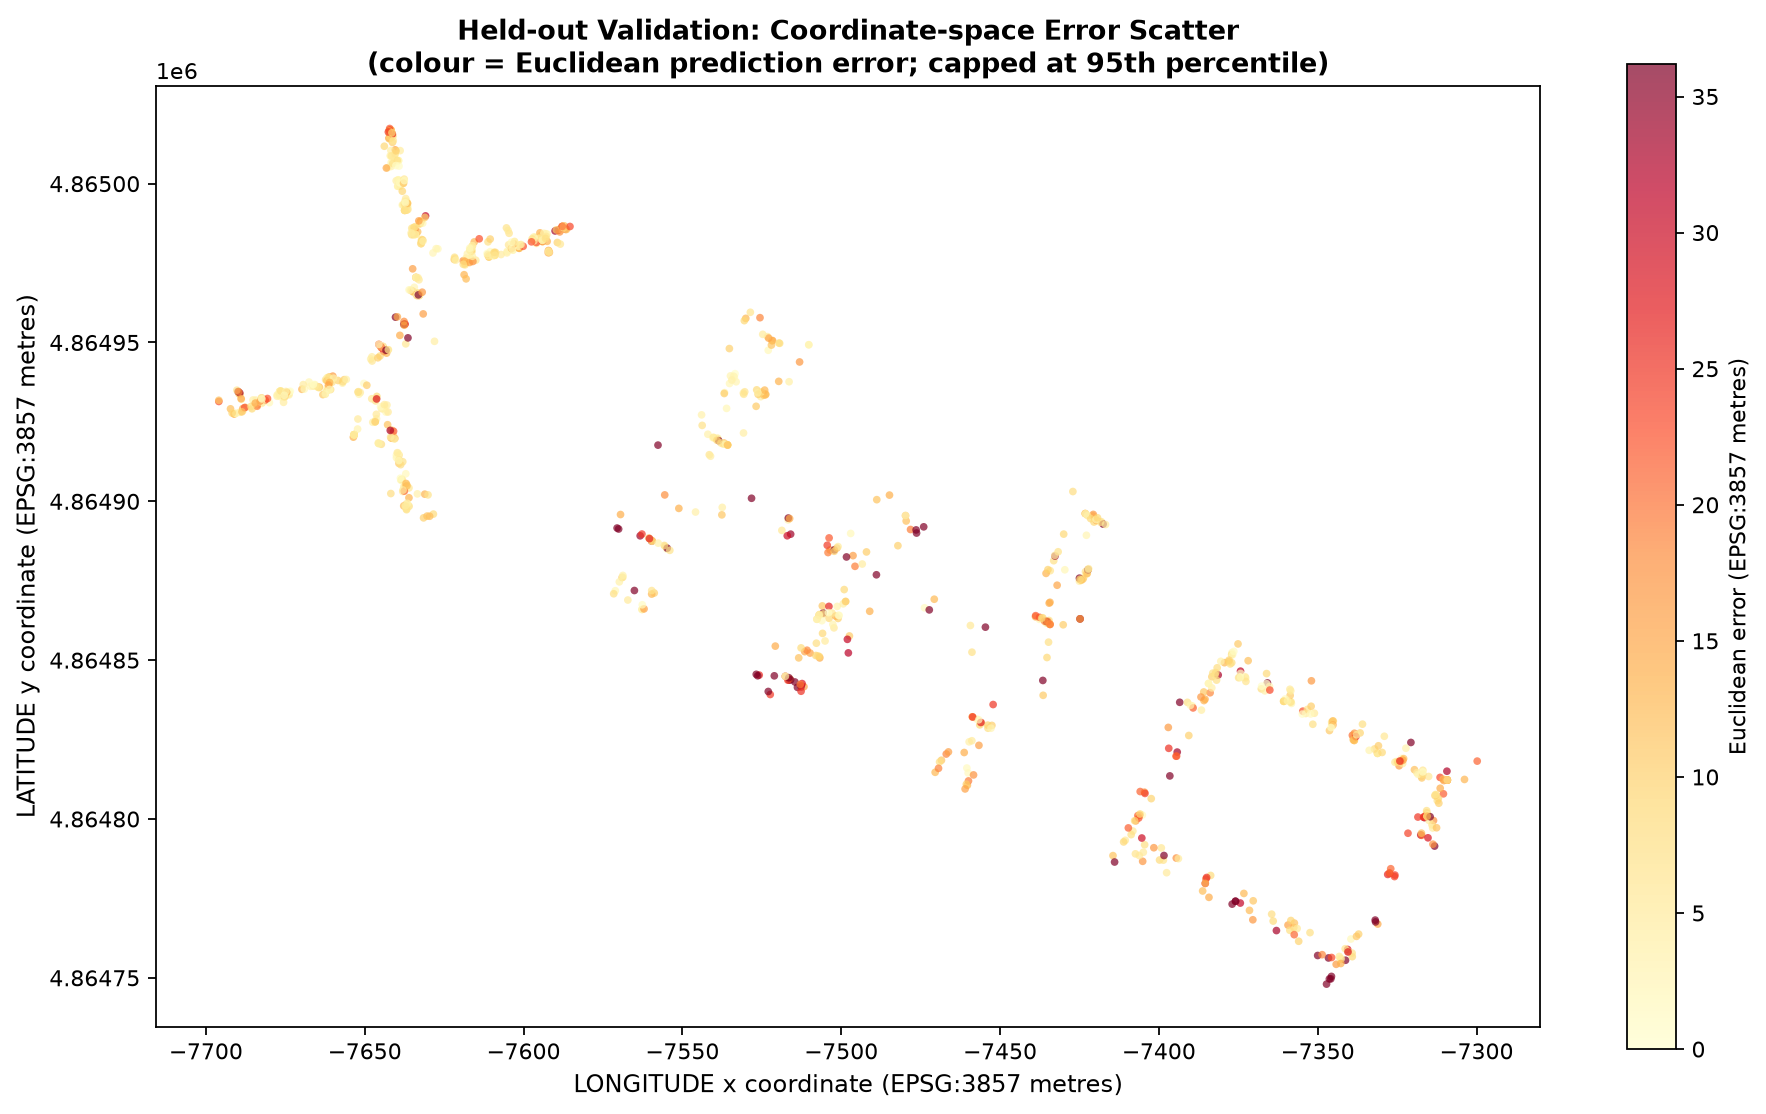
\includegraphics[width=0.94\columnwidth]{../data/figures/ml_04_coordinate_error_map.png}
  \caption{Held-out coordinate-space error scatter. Color encodes Euclidean prediction error; axes and error legend use the notebook's EPSG:3857 assumption. This is not a geographic basemap.}
  \label{fig:errormap}
\end{figure}

\subsection{Hierarchical evaluation}
Building and floor are predicted independently, so a correct floor code does not by itself imply the correct building--floor location. The integration notebook joins predictions using a composite source-partition and row-ID key, verifies key uniqueness, row coverage and true-label agreement, and recomputes the task metrics from the row-level outputs. It then evaluates exact joint building--floor correctness. On the 1,111 held-out rows, both labels are correct for 986 records (88.75\%).

Among held-out rows with both labels correct, mean coordinate error is 10.00 coordinate units. For 122 rows with a correct building but incorrect floor, it is 23.27 units; the two rows with an incorrect building but correct floor have mean error 44.31; one row with both labels incorrect has error 77.04. The latter groups are very small, so their means are descriptive only.

\begin{table}[!t]
\centering
\caption{Held-out hierarchical outcomes and coordinate error by classification correctness.}
\label{tab:hierarchy}
\begin{tabularx}{\columnwidth}{Xrrr}
\toprule
Building/floor outcome & Rows & Share & Mean coordinate error \\
\midrule
Both correct & 986 & 88.75\% & 10.00 \\
Building correct, floor wrong & 122 & 10.98\% & 23.27 \\
Building wrong, floor correct & 2 & 0.18\% & 44.31 \\
Both wrong & 1 & 0.09\% & 77.04 \\
\bottomrule
\end{tabularx}
\end{table}


\section{Limitations}
\begin{itemize}
  \item \textbf{Partition scope:} the split follows the supplied dataset and the internal building/floor/space grouping protocol. Fingerprint overlap and repeated positions may remain across partitions.
  \item \textbf{Coordinate reference:} EPSG:3857 and metre units are notebook assumptions; a source-of-truth CRS declaration is absent. Projection-scale correction is not applied.
  \item \textbf{Model search:} the searches are compact, fixed grids evaluated on one internal split; there is no repeated cross-validation or uncertainty interval.
  \item \textbf{Separate targets:} building, floor, and coordinates are learned independently. Their outputs can disagree, and no joint constraint enforces a valid building--floor combination or coordinate region.
  \item \textbf{Data imbalance and duplicates:} floor representation is uneven, particularly for floor 4. Exact duplicate rows and all-absent training examples were retained; their influence is not separately ablated.
  \item \textbf{Algorithm comparison:} Random Forest is the implemented estimator family. The reported results do not establish that it is better than XGBoost or other alternatives.
\end{itemize}

\section{Conclusion}
The pipeline combines train-only RSSI preprocessing with independent Random Forest predictors for building, floor, and coordinates. On the supplied held-out partition, accuracies were 99.73\% and 88.93\%, with mean coordinate error of 11.58 recorded units. These results do not establish performance on unseen fingerprints; the coordinate reference remains unverified.

\small
\begin{thebibliography}{9}
\bibitem{dawes2011}
B. Dawes and K.-W. Chin, ``A comparison of deterministic and probabilistic methods for indoor localization,'' \emph{Journal of Systems and Software}, vol. 84, no. 3, pp. 442--451, Mar. 2011, doi: \href{https://doi.org/10.1016/j.jss.2010.11.888}{10.1016/j.jss.2010.11.888}.

\bibitem{hechan2016}
S. He and S.-H. G. Chan, ``Wi-Fi fingerprint-based indoor positioning: Recent advances and comparisons,'' \emph{IEEE Communications Surveys \& Tutorials}, vol. 18, no. 1, pp. 466--490, 1st Quart. 2016, doi: \href{https://doi.org/10.1109/COMST.2015.2464084}{10.1109/COMST.2015.2464084}.

\bibitem{song2019}
X. Song, X. Fan, C. Xiang, Q. Ye, L. Liu, Z. Wang, X. He, and G. Fang, ``A novel convolutional neural network based indoor localization framework with WiFi fingerprinting,'' \emph{IEEE Access}, vol. 7, pp. 110698--110709, 2019, doi: \href{https://doi.org/10.1109/ACCESS.2019.2933921}{10.1109/ACCESS.2019.2933921}.

\bibitem{torres2014}
J. Torres-Sospedra, R. Montoliu, A. Mart\'{i}nez-Us\'{o}, J. P. Avariento, T. J. Arnau, M. Benedito-Bordonau, and J. Huerta,
``UJIIndoorLoc: A new multi-building and multi-floor database for WLAN fingerprint-based indoor localization problems,''
in \emph{Proc. 2014 International Conference on Indoor Positioning and Indoor Navigation (IPIN)}, Busan, Republic of Korea, 2014, pp. 261--270, doi: \href{https://doi.org/10.1109/IPIN.2014.7275492}{10.1109/IPIN.2014.7275492}.

\bibitem{uci}
UCI Machine Learning Repository, ``UJIIndoorLoc,'' dataset 310, doi: \href{https://doi.org/10.24432/C5MS59}{10.24432/C5MS59}. Available: \url{https://archive.ics.uci.edu/dataset/310/ujiindoorloc}.

\bibitem{breiman2001}
L. Breiman, ``Random forests,'' \emph{Machine Learning}, vol. 45, pp. 5--32, 2001, doi: \href{https://doi.org/10.1023/A:1010933404324}{10.1023/A:1010933404324}.
\end{thebibliography}

\end{document}
